\subsection{Factor Graphs}
\subsubsection{Factor Graphs in System Modelling}
Factor graphs provide a structured mathematical framework for representing probabilistic relationships between system variables and sensor measurements. Instead of expressing the full joint probability directly, the system is decomposed into a set of local factors, each representing a specific probabilistic constraint such as a process model, measurement model, or prior. The complete joint distribution is then expressed as a product of these factors, which preserves the underlying statistical dependencies while enabling efficient computation.  
\\ \\
In this work, the factor graph is used to describe the relationships between the microAmpere ASV state variables and their associated sensor observations. Each measurement, such as from the IMU or Side Scan Sonar, is represented as an independent factor, while the process model introduces constraints between consecutive time steps. 
This formulation provides a clear and modular way to combine heterogeneous sensor information within a unified probabilistic framework.  
\\ \\
The factor graph representation also serves as the foundation for optimization based estimation methods used in Smoothing and Mapping (SAM), where the sparsity of the graph structure allows efficient computation of the most probable state trajectory.

\begin{figure}[H]
    \centering
    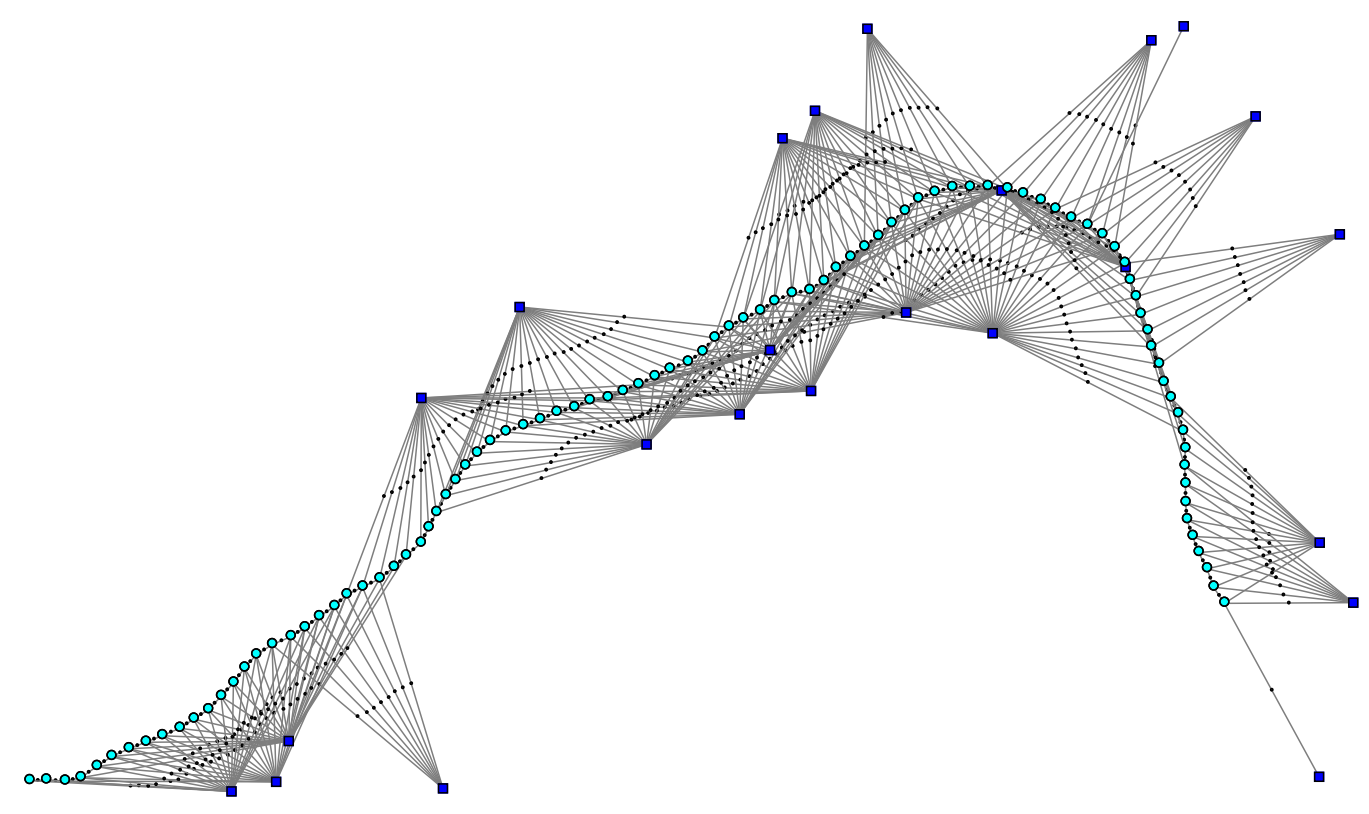
\includegraphics[width=0.9\linewidth]{Pictures/System_Modeling/Factor_Graphs/Example.png}
    \caption{Example of a factor graph in a simulated SLAM problem. Light blue circles represent the estimated robot trajectory, and dark blue squares represent observed landmarks. The connecting black edges/lines are factors, each defining a local probabilistic constraint between variables.\textsuperscript{\cite{factor_graphs}}}
    \label{fig:system-modeling-factor-graph-example}
\end{figure}

\newpage

\subsubsection{Mathematical Formulation}
A factor graph expresses the joint probability distribution of all system states as a product of smaller, locally defined functions. This can be written as:
$$
    p(\mathbf{x}) = \frac{1}{Z} \prod_{i=1}^{M} \phi_i(\mathbf{x}_i)
$$
where each factor $\phi_i(\mathbf{x}_i)$ represents a local probabilistic constraint involving only a subset of variables $\mathbf{x}_i$, and $Z$ is a normalization constant.  
\\ \\
In system modelling, these factors describe relationships such as motion models $f(\mathbf{x}, \mathbf{u})$ that connect consecutive states (See Equation \ref{eq:kinematics-motion-model}), measurement models $h(\mathbf{x})$ linking states to sensor observations (For example processed Side Scan Sonar 2D image), and prior terms that encode initial conditions. This factorization captures the conditional independence structure of the system and enables efficient and modular computation within probabilistic estimation frameworks.



\subsubsection{Integration in the System Model}
In this project, factor graphs are used to represent the complete state estimation problem by combining the INS motion model with processed measurements from the Side Scan Sonar within a unified probabilistic framework. The motion model defines the dynamic constraints between time steps, while the sonar derived landmark observations add measurement factors that update and refine the estimated trajectory within the overall system model.
